% !TEX root = ../main.tex

Chapter~1 stated the problem and the proved results.
This chapter explains how a program can measure connectivity in every variant, check small graphs one by one, and search for dense examples.
No result in this thesis depends on the output of this program.
Its output for $n,m\le7$ is printed in \Cref{app:program}.
\Cref{sec:certificates} shows how an output can be checked without reading the code.

The program is one Python file of about $750$ lines, \texttt{program/erdos915.py}.
It uses the library \texttt{networkx} for maximum flows, and the programs \texttt{geng}, \texttt{directg} and \texttt{genbg} of \texttt{nauty} to list graphs.
This chapter prints the main parts of the program, each next to the idea it implements.
The remaining parts, such as the imports and small helper functions, are in \Cref{app:program}, so every line of the program is printed once.
The names in the code follow the words of the text.
\Cref{fig:spine} shows the structure of the program.
\begin{figure}[ht]
\centering
\spinediagram
\caption{One model feeds the max-flow computation. Exhaustive search uses it to find exact values, heuristic search uses it to find dense examples, and the check with \texttt{nauty} uses it to show that no feasible graph has one edge more than the densest one found (\Cref{sec:one-more}).}
\label{fig:spine}
\end{figure}

\section{Modelling}
The program treats all eight models in one way.
A model is described by four facts: whether it is directed, whether edges may repeat, the edge size $r$, and, for directed hypergraphs, the allowed numbers of tails.
A graph is the case $r=2$.
The program runs each directed hypergraph model in three versions, forward, backward and general (\Cref{sec:variants}), so \texttt{ALL\_MODELS} lists twelve entries for the eight models.
The separation, edge or vertex, is a separate choice, so the eight models give the sixteen problems.
A \texttt{Problem} bundles a model, a separation, the number of vertices $n$ and the threshold $m$, and every function below takes one (\Cref{lst:models}).

\programpart{models}{The models, with three versions of each directed hypergraph model, and the two separations.}

Every edge is stored as a hyperedge: its vertices, and its tails if the model is directed.
An ordinary edge $uv$ is the hyperedge $\{u,v\}$ without tails, and an arc $u\to v$ is the hyperedge $\{u,v\}$ with tail $u$.
A route may enter a hyperedge only at one of its \emph{entry vertices}, and leave it only at one of its \emph{exit vertices} (\texttt{entry\_vertices} and \texttt{exit\_vertices} in the code).
In an undirected hyperedge every vertex is both. In a directed one only the tails are entries and only the heads are exits.
A candidate graph is a table that gives every possible hyperedge its multiplicity.
We call the models without repeated edges \emph{simple models}, and the models with repeated edges \emph{multi models}.
In a simple model every multiplicity is $0$ or $1$. In a multi model it is at most $m-1$, since $m$ copies of one edge already give $m$ disjoint routes (\Cref{lst:hyperedges}).
\Cref{fig:matrix-rep} shows two such tables.

\programpart{hyperedges}{Hyperedges, the list of all possible hyperedges, and the largest useful multiplicity.}



\begin{figure}[ht]
\centering
\newcommand{\hetable}[1]{%
  {\small\renewcommand{\arraystretch}{1.15}%
  \begin{tabular}{@{}ccc@{}}
  \texttt{\color{codeConstant}TAILS} & \texttt{\color{codeConstant}MEMBERS} & copies\\ \midrule
  #1
  \end{tabular}}}
\begin{tikzpicture}[>=Stealth]
% ---- (a) directed multigraph -> its hyperedge table ----
\node[vertex] (A) at (0,   0)   {$1$};
\node[vertex] (B) at (2.0, 0)   {$2$};
\node[vertex] (C) at (1.0, 1.7) {$3$};
\draw[arc] (A) to[bend left=15]  (B);
\draw[arc] (A) to[bend right=15] (B);
\draw[arc] (B) to[bend left=15]  (C);
\draw[arc] (C) to[bend left=15] (B);
\draw[arc] (A) -- (C);
\node[font=\small] at (1.0, -0.8) {directed multigraph};
\node at (3.4, 0.55) {$\longrightarrow$};
\node at (6.2, 0.55) {\hetable{
  $\{1\}$ & $\{1,2\}$ & ${\color{vertexred}\mathbf 2}$ \\
  $\{1\}$ & $\{1,3\}$ & $1$ \\
  $\{2\}$ & $\{2,3\}$ & $1$ \\
  $\{3\}$ & $\{2,3\}$ & $1$ \\}};
\node[font=\small] at (1.0, -1.25) {(a)};
% ---- (b) directed hypergraph -> its hyperedge table ----
\begin{scope}[yshift=-3.9cm]
  \coordinate (p1) at (0.0, 0.6);
  \coordinate (p2) at (0.0,-0.6);
  \coordinate (p3) at (1.1, 0.0);
  \coordinate (p4) at (2.2, 0.6);
  \coordinate (p5) at (2.2,-0.6);
  \begin{scope}[on background layer]
    \draw[metro, metroA, -{Stealth[length=2.6mm]}, shorten >=2mm, shorten <=1.4mm] (p3) -- (p1);
    \draw[metro, metroA, -{Stealth[length=2.6mm]}, shorten >=2mm, shorten <=1.4mm] (p3) -- (p2);
    \draw[metro, metroB, -{Stealth[length=2.6mm]}, shorten >=2mm, shorten <=1.4mm] (p3) -- (p5);
    \draw[metro, metroB, -{Stealth[length=2.6mm]}, shorten >=2mm, shorten <=1.4mm] (p4) -- (p5);
  \end{scope}
  \foreach \p/\lbl in {p1/1,p2/2,p3/3,p4/4,p5/5} {\node[smallvertex] at (\p) {$\lbl$};}
  \node[font=\small] at (1.1,-1.15) {directed hypergraph};
  \node at (3.4, 0.0) {$\longrightarrow$};
  \node at (6.2, 0.0) {\hetable{
    {\color{metroA}$\{\mathbf 3\}$} & {\color{metroA}$\{1,2,3\}$} & $1$ \\
    {\color{metroB}$\{\mathbf 3,\mathbf 4\}$} & {\color{metroB}$\{3,4,5\}$} & $1$ \\}};
  \node[font=\small] at (1.1,-1.6) {(b)};
\end{scope}
\end{tikzpicture}
\caption{The program stores every model in one way: a table that gives each hyperedge its number of copies. (a) A directed multigraph. The arc $u\to v$ is the hyperedge with members $\{u,v\}$ and tail $u$, and the two parallel arcs from $1$ to $2$ are one row with $2$ copies. (b) A directed $3$-uniform hypergraph in the general model. Each hyperedge records its tails and its three members: the red one has tail $3$, the blue one has tails $3$ and $4$ and head $5$. In an undirected model there are no tails. A hyperedge that does not occur has $0$ copies and is left out.}
\label{fig:matrix-rep}
\end{figure}

\section{Measuring}
Every search below needs $\lec^{\max}$ or $\kap^{\max}$ of a candidate graph.
This section explains how the program computes them.

To compute $\lec(u,v)$ we use a maximum flow.
In a network every link has a capacity, and a \emph{maximum flow} is the largest amount that can be sent from $u$ to $v$.
We give each pair of vertices a link with capacity $\mu(u,v)$.
In a digraph the link has a direction. In an undirected graph it can be used in both directions.
The max-flow min-cut theorem of Ford and Fulkerson \cite{FordFulkerson56} says that the maximum flow equals the smallest capacity of a cut.
By Menger's theorem, this is $\lec(u,v)$.
So computing a maximum flow computes $\lec(u,v)$.
We call this the \emph{max-flow computation}.


\subsection{Transformations}
The max-flow computation works on one kind of network for all sixteen problems.

Every hyperedge, including an ordinary edge, becomes a \emph{gate} (\Cref{fig:hyper-gadget}).
The gate has an entry node and an exit node, joined by one arc whose capacity is the multiplicity of the hyperedge.
Each vertex of the hyperedge gets an arc of unlimited capacity to the entry node and one from the exit node.
So the arc inside the gate is the only bottleneck.
For a directed hyperedge, only the tails have an arc to the entry, and only the heads have an arc from the exit (\Cref{fig:dir-hyper-gadget}).
So a route must go from a tail to a head.
\Cref{thm:menger-hyper} shows that the maximum flow in this network is the number of hyperedge-disjoint Berge routes.
\Cref{fig:hyper-gadget-example} shows an example.

Every vertex $v$ is split into two nodes $v^{\mathrm{in}}$ and $v^{\mathrm{out}}$, joined by one arc (\Cref{fig:vertex-split}).
Routes arrive at $v^{\mathrm{in}}$ and leave from $v^{\mathrm{out}}$.
For vertex separation this arc has capacity one, so at most one route can pass through $v$.
For edge separation its capacity is unlimited, and it changes nothing.
The gates keep their capacity, so parallel copies still give separate routes, as in the incidence convention of \Cref{sec:incidence-convention}.
\Cref{lst:network} builds this network.

\programpart{network}{The flow network: split vertices and one gate per hyperedge.}

The number of disjoint routes from $u$ to $v$ is the maximum flow from $u^{\mathrm{out}}$ to $v^{\mathrm{in}}$ (\Cref{lst:measure}).
A graph is feasible when this number is below $m$ for every pair, ordered in directed models.
The flow may stop as soon as it reaches $m$, since a larger value changes nothing. This is the \texttt{stop\_at} argument.

\programpart{measure}{Counting disjoint routes, and the feasibility test.}

\begin{figure}[htbp]
\centering
% Printed legibility: this picture holds two 8-unit panels side by side, so
% every extra centimetre of gap or of resize headroom is paid for twice over in
% label size. The gap is kept tight, the box is given the full text width, and
% the station and gate fonts are stepped up, which together lift the smallest
% label from about 5.4pt to roughly 9pt on paper.
\resizebox{\textwidth}{!}{%
\begin{tikzpicture}[scale=0.92, >=Stealth,
   metro/.append style={line width=3.0pt},
   metrostop/.append style={font=\small\bfseries, minimum size=6.6mm},
   faded/.style={metro, opacity=0.35, line width=2.2pt},
   flow/.style={line width=1.2pt, black!88, line cap=round,
                preaction={draw, line width=3.0pt, white}},
   gate/.style={circle, fill=white, draw=black!30, line width=0.6pt,
                inner sep=0.4pt, minimum size=13.5pt, font=\small}]
\def\stations{%
  \coordinate (Sa) at (0,0);  \coordinate (Sc) at (2,2);  \coordinate (Sd) at (6,2);
  \coordinate (Se) at (0,4);  \coordinate (Sj) at (8,4);  \coordinate (Sl) at (2,6);
  \coordinate (Sm) at (6,6);  \coordinate (Sn) at (0,8);}
% Every station carries its own letter, since the captions name hyperedges and
% routes by those letters.  The chosen pair also carries its role name, u or v,
% in blue just outside the station.
\def\drawstops{%
  \foreach \id/\lab in {Sa/a,Sc/c,Sd/d,Se/e,Sj/j,Sl/l,Sm/m,Sn/n}
     {\node[metrostop] at (\id) {$\lab$};}
  \node[font=\small\bfseries, text=KULblauw1] at ($(Se)+(-0.62,0.52)$) {$u$};
  \node[font=\small\bfseries, text=KULblauw1] at ($(Sm)+(0.62,0.52)$) {$v$};}
% --- panel (a): the hypergraph, every hyperedge vertex to vertex ---
\begin{scope}
  \stations
  \begin{scope}[on background layer]
    \draw[metro, metroA] (Se) -- (Sa);
    \draw[metro, metroA] (Sa) -- (Sd);
    \draw[metro, metroB] (Sn) -- (Sm);
    \draw[metro, metroB] (Sm) -- (Sj);
    \draw[metro, metroC] ($(Se)+(0.14,-0.14)$) -- ($(Sl)+(0.14,-0.14)$);
    \draw[metro, metroC] (Sl) -- (Sc);
    \draw[metro, metroD] (Se) -- (Sd);
    \draw[metro, metroD] (Sd) -- (Sm);
    \draw[metro, metroF] (Sn) -- (Se);
    \draw[metro, metroF] (Se) -- (Sl);
    \draw[metro, metroH] ($(Se)+(-0.14,0.14)$) -- ($(Sl)+(-0.14,0.14)$);
    \draw[metro, metroH] (Sl) -- (Sm);
    \draw[metro, metroG] (Sm) -- (Sc);
    \draw[metro, metroG] (Sc) -- (Sj);
    \draw[metro, metroE] (Sl) -- (Sd);
    \draw[metro, metroE] (Sd) -- (Sj);
  \end{scope}
  \drawstops
  \node[font=\small] at (4,-1.4) {(a)};
\end{scope}
% --- panel (b): the helper-point flow network for the pair u, v ---
\begin{scope}[xshift=9.6cm]
  \stations
  \coordinate (Helc) at (1,3);
  \coordinate (Hmcj) at (5,4);
  \coordinate (Hedm) at (3,3.7);
  \coordinate (Helm) at (1.6,6.7);
  \coordinate (Hnel) at (0.50,6.00);
  \coordinate (Hnmj) at (3.27,7.81);
  \begin{scope}[on background layer]
    \draw[faded, metroA] (Se) -- (Sa);
    \draw[faded, metroA] (Sa) -- (Sd);
    \draw[faded, metroB] (Sn) -- (Sm);
    \draw[faded, metroB] (Sm) -- (Sj);
    \draw[faded, metroC] ($(Se)+(0.14,-0.14)$) -- ($(Sl)+(0.14,-0.14)$);
    \draw[faded, metroC] (Sl) -- (Sc);
    \draw[faded, metroD] (Se) -- (Sd);
    \draw[faded, metroD] (Sd) -- (Sm);
    \draw[faded, metroF] (Sn) -- (Se);
    \draw[faded, metroF] (Se) -- (Sl);
    \draw[faded, metroH] ($(Se)+(-0.14,0.14)$) -- ($(Sl)+(-0.14,0.14)$);
    \draw[faded, metroH] (Sl) -- (Sm);
    \draw[faded, metroG] (Sm) -- (Sc);
    \draw[faded, metroG] (Sc) -- (Sj);
    \draw[faded, metroE] (Sl) -- (Sd);
    \draw[faded, metroE] (Sd) -- (Sj);
  \end{scope}
  \draw[flow] (Se) -- (Helc);
  \draw[flow] (Helc) -- (Sc);
  \draw[flow] (Sc) -- (Hmcj);
  \draw[flow] (Hmcj) -- (Sm);
  \draw[flow] (Se) -- (Hedm);
  \draw[flow] (Hedm) -- (Sm);
  \draw[flow] (Se) -- (Helm);
  \draw[flow] (Helm) -- (Sm);
  \draw[flow] (Se) -- (Hnel);
  \draw[flow] (Hnel) -- (Sn);
  \draw[flow] (Sn) -- (Hnmj);
  \draw[flow] (Hnmj) -- (Sm);
  % dotted leg from each gate to the hyperedge's unused third member
  \draw[densely dotted, line width=1pt, opacity=0.7, shorten >=3mm, metroC] (Helc) -- (Sl);
  \draw[densely dotted, line width=1pt, opacity=0.7, shorten >=3mm, metroG] (Hmcj) -- (Sj);
  \draw[densely dotted, line width=1pt, opacity=0.7, shorten >=3mm, metroD] (Hedm) -- (Sd);
  \draw[densely dotted, line width=1pt, opacity=0.7, shorten >=3mm, metroH] (Helm) -- (Sl);
  \draw[densely dotted, line width=1pt, opacity=0.7, shorten >=3mm, metroF] (Hnel) -- (Sl);
  \draw[densely dotted, line width=1pt, opacity=0.7, shorten >=3mm, metroB] (Hnmj) -- (Sj);
  \node[gate] at (Helc) {$h_{\textcolor{metroC}{\bullet}}$};
  \node[gate] at (Hmcj) {$h_{\textcolor{metroG}{\bullet}}$};
  \node[gate] at (Hedm) {$h_{\textcolor{metroD}{\bullet}}$};
  \node[gate] at (Helm) {$h_{\textcolor{metroH}{\bullet}}$};
  \node[gate] at (Hnel) {$h_{\textcolor{metroF}{\bullet}}$};
  \node[gate] at (Hnmj) {$h_{\textcolor{metroB}{\bullet}}$};
  \drawstops
  \node[font=\small] at (4,-1.4) {(b)};
\end{scope}
\end{tikzpicture}}
\caption[The gate network of a hypergraph]{(a) An undirected $3$-uniform hypergraph. (b) The relevant part of its gate network for the pair $u,v$. The four black routes use pairwise disjoint sets of gates, so $\lec(u,v)\ge4$. The vertex $v$ lies in only four hyperedges, and removing those four hyperedges separates $u$ from $v$, so $\lec(u,v)\le4$. Hence $\lec(u,v)=4$. Each gate is drawn as one point. A dotted line joins a gate to the third vertex of its hyperedge, which the route does not use.}
\label{fig:hyper-gadget-example}
\end{figure}

% Printed legibility: three panels across at 0.32\textwidth shrank each picture
% to roughly 0.58 of natural size and its labels to under 5pt. Stacking them
% one per row at 0.70\textwidth reverses that, drawing each slightly larger
% than natural instead.
\begin{figure}[ht]
\centering
\begin{subfigure}[b]{0.70\textwidth}
\centering
\resizebox{\linewidth}{!}{%
\begin{tikzpicture}[>=Stealth]
\node[vertex] (v) at (1.0, 0) {$v$};
\draw[->, edge] (0.0,  0.6) -- (v);
\draw[->, edge] (0.0, -0.6) -- (v);
\draw[->, edge] (v) -- (2.0,  0.6);
\draw[->, edge] (v) -- (2.0, -0.6);
\draw[->, very thick, color=KULblauw3b] (2.8, 0) -- (3.8, 0);
\node[smallvertex, minimum size=8mm] (vi) at (5.0, 0) {$v^{\mathrm{in}}$};
\node[smallvertex, minimum size=8mm] (vo) at (7.0, 0) {$v^{\mathrm{out}}$};
\draw[->, edge, color=KULblauw3b] (vi) -- node[above, font=\scriptsize]{capacity $1$} (vo);
\draw[->, edge] (4.0,  0.6) -- (vi);
\draw[->, edge] (4.0, -0.6) -- (vi);
\draw[->, edge] (vo) -- (8.0,  0.6);
\draw[->, edge] (vo) -- (8.0, -0.6);
\end{tikzpicture}}
\caption{Splitting each vertex $v$ into $v^{\mathrm{in}}$ and $v^{\mathrm{out}}$, joined by an arc of capacity one, turns vertex-disjoint routes into arc-disjoint routes. Only this inner arc has capacity one.}
\label{fig:vertex-split}
\end{subfigure}

\bigskip
\begin{subfigure}[b]{0.70\textwidth}
\centering
\resizebox{\linewidth}{!}{%
\begin{tikzpicture}[>=Stealth]
\coordinate (a) at (0.0, 0.0); \coordinate (b) at (1.0, 0.0); \coordinate (c) at (2.0, 0.0);
\begin{scope}[on background layer]\draw[metro, metroA] (a)--(b)--(c);\end{scope}
\node[smallvertex] at (a) {$a$}; \node[smallvertex] at (b) {$b$}; \node[smallvertex] at (c) {$c$};
\draw[->, very thick, color=KULblauw3b] (2.85, 0.0) -- (3.95, 0.0);
\begin{scope}[xshift=4.6cm]
% members in a column, gate pair beside them: every member sends one uncapped
% arc into e^- and receives one uncapped arc out of e^+.
\node[smallvertex] (a2) at (0.0,  1.30) {$a$};
\node[smallvertex] (b2) at (0.0,  0.00) {$b$};
\node[smallvertex] (c2) at (0.0, -1.30) {$c$};
\node[hnode, fill=metroA!70, minimum size=15pt] (em) at (2.05,  0.62) {$e^-$};
\node[hnode, fill=metroA!70, minimum size=15pt] (ep) at (2.05, -0.62) {$e^+$};
% into the gate
\draw[gdirfaint] (a2) to[bend left=8]  node[above, font=\scriptsize, text=black!55, pos=0.55]{$\infty$} (em);
\draw[gdirfaint] (b2) to[bend left=10] (em);
\draw[gdirfaint] (c2) to[bend left=22] (em);
% out of the gate
\draw[gdirfaint] (ep) to[bend left=22] (a2);
\draw[gdirfaint] (ep) to[bend left=10] (b2);
\draw[gdirfaint] (ep) to[bend left=8]  node[below, font=\scriptsize, text=black!55, pos=0.45]{$\infty$} (c2);
% the one bottleneck
\draw[gdir, line width=1.6pt, color=KULblauw3b] (em) -- node[right, font=\scriptsize]{capacity $\mu$} (ep);
\end{scope}
\end{tikzpicture}}
\caption{Transform a hyperedge into a gate with capacity equal to the multiplicity of the hyperedge.}
\label{fig:hyper-gadget}
\end{subfigure}

\bigskip
\begin{subfigure}[b]{0.70\textwidth}
\centering
\resizebox{\linewidth}{!}{%
\begin{tikzpicture}[>=Stealth, gatearc/.style={gdir}]
\node[smallvertex] (a) at (0.0, 1.05) {$a$}; \node[smallvertex] (b) at (-0.85, -0.55) {$b$}; \node[smallvertex] (c) at (0.85, -0.55) {$c$};
\begin{scope}[on background layer]
  \draw[metro, metroB, -{Stealth[length=2.8mm]}, shorten >=2mm, shorten <=1.4mm] (a) -- (b);
  \draw[metro, metroB, -{Stealth[length=2.8mm]}, shorten >=2mm, shorten <=1.4mm] (a) -- (c);
\end{scope}
\draw[->, very thick, color=KULblauw3b] (2.4, 0.1) -- (3.5, 0.1);
\begin{scope}[xshift=5.4cm]
  \node[smallvertex] (a2) at (0.0, 1.55) {$a$};
  \node[hnode, fill=metroB!70, minimum size=15pt] (gm) at (0.0,  0.52) {$e^-$};
  \node[hnode, fill=metroB!70, minimum size=15pt] (gp) at (0.0, -0.62) {$e^+$};
  \node[smallvertex] (b2) at (-1.05, -1.55) {$b$}; \node[smallvertex] (c2) at (1.05, -1.55) {$c$};
  \draw[gdirfaint] (a2) -- node[right, font=\scriptsize, text=black!60]{$\infty$} (gm);
  \draw[gdir, line width=1.6pt, color=KULblauw3b] (gm) -- node[right, font=\scriptsize]{capacity $\mu$} (gp);
  \draw[gdirfaint] (gp) -- node[left, pos = 0.3, font=\scriptsize, text=black!60]{$\infty$} (b2);
  \draw[gdirfaint] (gp) -- node[right, pos = 0.3, font=\scriptsize, text=black!60]{$\infty$} (c2);
\end{scope}
\end{tikzpicture}}
\caption{A directed hyperedge with one tail and two heads is transformed into a gate. This gate has capacity equal to the multiplicity of the hyperedge and every route must enter at the tail and leave at a head. With several tails, each tail has an arc to $e^-$.}
\label{fig:dir-hyper-gadget}
\end{subfigure}
\caption{The building blocks of the max-flow computation: vertex splitting, hyperedge gates and directed hyperedge gates.}
\label{fig:checker-gadgets}
\end{figure}

\section{Checking every graph with a fixed number of vertices}\label{sec:certification-standard}
The program stores a graph as a table that gives each possible hyperedge its number of copies (\Cref{fig:matrix-rep}).
The possible hyperedges depend on the model:
\begin{itemize}
\item in a graph, the $\binom n2$ pairs $\{u,v\}$,
\item in a digraph, the $n(n-1)$ ordered pairs, one for each arc $u\to v$,
\item in an $r$-uniform hypergraph, the $\binom nr$ sets of $r$ vertices, called \emph{$r$-sets},
\item in a directed $r$-uniform hypergraph, an $r$-set together with a choice of which of its vertices are tails.
A forward hyperedge has one tail, so each $r$-set gives $r$ possible hyperedges.
A backward hyperedge has one head, which also gives $r$.
In the general model the tails form any non-empty proper subset, which gives $2^r-2$.
\end{itemize}
Each entry of the table is between $0$ and the largest multiplicity: $1$ in a simple model and $m-1$ in a multi model.
To find an exact value, the program must show that no table with more copies than the best feasible graph found is feasible.
If the search stops early, it gives only a lower bound.

\begin{figure}[ht]
    \centering
    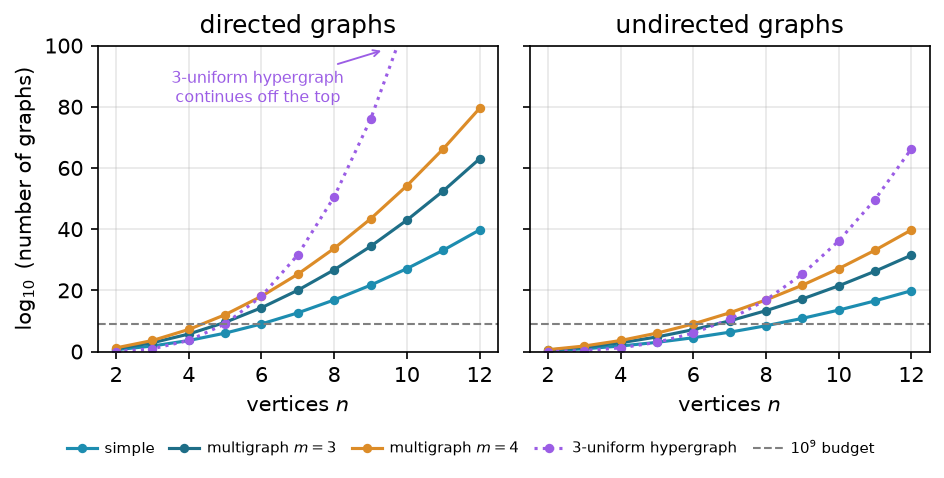
\includegraphics[width=\textwidth]{figures/complexity_growth.png}
    \caption{The number of candidates for blind enumeration, on a logarithmic scale. Every model passes $10^9$ candidates before $n=10$. Directed models grow fastest, because they have more entries to choose. The directed hypergraph curve is the forward model.}
    \label{fig:complexity}
\end{figure}

The number of vertices matters most.
The number of candidates is (values per entry) to the power (number of entries).
For graphs the number of entries grows like $n^2$, and for $r$-uniform hypergraphs like $n^r$.
A larger $m$ gives more values per entry.
Direction gives more entries, since both directions of a pair are chosen separately.
Directed hypergraphs have the most candidates, because each $r$-set carries several possible hyperedges.
The separation does not change the candidates. It only changes the test for each candidate.


So there are $2^{\binom n2}$ simple graphs and $2^{n(n-1)}$ simple digraphs on $n$ vertices.
With multiplicities at most $m-1$ there are $m^{\binom n2}$ multigraphs and $m^{n(n-1)}$ directed multigraphs.
\Cref{fig:complexity} shows how fast this grows.
The program uses two exact methods: a pruned search, for every model, and a check of the graphs with one edge more, for every model except directed hypergraphs.

\subsection{Pruned search}
A pruned search skips whole families of graphs.
Fix an order on the possible edges and decide them one at a time.
A partly built graph stands for all graphs that agree with it so far.
A pruning rule can discard this whole family.

The first rule uses that adding an edge never lowers connectivity.
If a partly built graph already breaks the condition, so does every way to complete it, and the branch is dropped.

The second rule bounds the size of every completion: the edges already placed, plus the number of undecided edges times the largest allowed multiplicity.
If this cannot beat the best graph found so far, the branch is dropped (\Cref{fig:prune}).

Both rules only drop graphs that are infeasible or cannot beat the best one.
So a finished pruned search gives the same answer as the full search.

\Cref{lst:exhaustive} decides the possible hyperedges one at a time, in a fixed order.
For each it tries $1, 2, \dots$ copies, and stops at the first number of copies that makes the graph infeasible, since more copies stay infeasible.
Then it also tries $0$ copies.
The test on \texttt{undecided} in \texttt{decide} is the second rule: if even all undecided hyperedges at full multiplicity cannot beat the best graph so far, the branch is dropped.
After the time limit the search stops and reports the best graph so far as a lower bound only.

\programpart{exhaustive}{The pruned exhaustive search.}

\begin{figure}[ht]
\centering
\begin{tikzpicture}[scale=1.0, >=Stealth,
   live/.style={gvertex, minimum size=5.5mm},
   dead/.style={gvsink, minimum size=5.5mm},
   bnd/.style={gvhub, minimum size=5.5mm},
   best/.style={gvertex, draw=vertexgreen!70!black, fill=vertexgreen!18, minimum size=5.5mm},
   br/.style={gline}]
  \node[live] (r) at (0,0) {};
  \node[live] (l) at (-2.2,-1.3) {};
  \node[live] (rr) at (2.2,-1.3) {};
  \draw[br] (r) -- node[above left, font=\scriptsize, pos=0.55]{add arc} (l);
  \draw[br] (r) -- node[above right, font=\scriptsize, pos=0.55]{skip arc} (rr);
  \node[best] (l1) at (-3.1,-2.7) {};
  \node[dead] (l2) at (-1.4,-2.7) {};
  \draw[br] (l)--(l1);
  \draw[line width=1pt, vertexred!60] (l)--(l2);
  \node[dead] (r1) at (1.3,-2.7) {};
  \node[bnd]  (r2) at (3.1,-2.7) {};
  \draw[line width=1pt, vertexred!60] (rr)--(r1);
  \draw[line width=1pt, vertexorange!70] (rr)--(r2);
  \node[font=\scriptsize, vertexgreen!50!black, align=center] at (-3.1,-3.5) {best\\feasible};
  \node[font=\scriptsize, vertexred, align=center] at (-1.4,-3.5) {infeasible\\(prune)};
  \node[font=\scriptsize, vertexred, align=center] at (1.3,-3.5) {infeasible\\(prune)};
  \node[font=\scriptsize, vertexorange!80!black, align=center] at (3.1,-3.5) {cannot beat\\best (prune)};
\end{tikzpicture}
\caption{Each level of the search decides one arc. Partly built graphs that are already infeasible (red), and branches that cannot beat the best graph found so far (orange), are dropped.}
\label{fig:prune}
\end{figure}

\subsection{Checking one edge more}\label{sec:one-more}
The pruned search meets every graph many times.
Renaming the vertices of a graph gives a graph with the same number of edges and the same connectivities, so the renamed graph is feasible exactly when the original is.
A graph on $n$ vertices has up to $n!$ renamings, so most of the work of the pruned search repeats work it has already done.

The second method avoids this.
It starts from a feasible graph with $L$ edges, found by the pruned search or by the heuristic search of \Cref{sec:heuristic}.
Removing an edge creates no new route, so it never makes a feasible graph infeasible.
So if a feasible graph with more than $L$ edges existed, removing edges from it one at a time would give a feasible graph with exactly $L+1$ edges.
It is therefore enough to check every graph with exactly $L+1$ edges.
If none of them is feasible, $L$ is the maximum.
If one of them is feasible, the program keeps it, replaces $L$ by $L+1$, and checks again.

To list these graphs, each only once up to renaming the vertices, the program uses the toolkit \texttt{nauty} of McKay and Piperno \cite{McKayPiperno14}, to which Prof.\ Jan Goedgebeur pointed us.
Three of its programs cover six of the eight models:
\begin{itemize}
\item \texttt{geng} lists the simple graphs on $n$ vertices with a given number of edges,
\item \texttt{directg} takes each graph from \texttt{geng} and directs each of its edges one way or both ways, which lists the simple digraphs,
\item \texttt{genbg} lists bipartite graphs: graphs whose vertices are split into two sides, with every edge joining the two sides. A hypergraph is the bipartite graph with the $n$ vertices on one side and the hyperedges on the other side, each hyperedge joined to its $r$ vertices. With the option \texttt{-z} no two hyperedges have the same vertices, so the hypergraph is simple.
\end{itemize}
\texttt{nauty} has no program that lists directed hypergraphs, so the program does not run this check for them. Their exact values come from the pruned search only.

\texttt{nauty} lists simple graphs only.
The \emph{support} of a multigraph is the simple graph of the pairs, or $r$-sets, that carry at least one copy.
For a multi model the program takes each support from \texttt{nauty} and chooses the number of copies of each of its edges, between $1$ and $m-1$, with $L+1$ copies in total.
A support with $k$ edges carries between $k$ and $k(m-1)$ copies, so only supports with between $\lceil (L+1)/(m-1)\rceil$ and $L+1$ edges are listed.
Renaming the vertices of a multigraph renames its support in the same way, so every multigraph with $L+1$ edges arises from some listed support.
Two choices of copies on the same support can give the same multigraph up to renaming. This repeats work but does not affect the result.
In a simple model the support is the graph itself, with one copy of each edge.
The copies are chosen one edge at a time, as in the pruned search: the program tries $1, 2, \dots$ copies and stops at the first number that makes the graph infeasible, since more copies stay infeasible.

\Cref{lst:nauty} builds the \texttt{nauty} commands and reads their output one support at a time, so the check can stop at its time limit before all supports are listed.
For digraphs two programs work together: \texttt{geng} passes every graph it lists to \texttt{directg}, which directs its edges.
The program counts the list as complete only if both programs exit normally.
If \texttt{geng} failed and \texttt{directg} did not, \texttt{directg} would receive no graphs and exit normally. The list would then look empty, and the check would report a value as exact without having checked anything.
\Cref{lst:larger} chooses the copies, and repeats the check while it finds a feasible graph with one edge more.

\programpart{nauty}{Listing the supports with \texttt{geng}, \texttt{directg} and \texttt{genbg} from \texttt{nauty}.}

\programpart{larger}{Checking every graph with one edge more.}

\section{The heuristic search}\label{sec:heuristic}
For larger $n$ the full search is impossible.
Instead we search for dense graphs in a guided way.
A \emph{heuristic} is a rule that moves the search towards better graphs.
The methods below also allow moves that make the graph worse, so that the search does not get stuck.

For graphs and digraphs, each candidate gets an \emph{energy}
\[
    \Phi(G) = -|E(G)| + \Lambda \cdot \max\bigl(0,\ c^{\max}(G) - (m - 1)\bigr).
\]
Here $c^{\max}(G)$ is $\lec^{\max}(G)$ or $\kap^{\max}(G)$, depending on the separation, and $\Lambda>0$ is a fixed penalty.
Low energy means many edges and no excess connectivity.
In the program $\Lambda$ is \texttt{PENALTY\_PER\_EXCESS\_ROUTE} (\Cref{lst:energy}).

\programpart{energy}{The energy of a candidate graph.}

The search starts from the empty graph and changes one multiplicity by one at each step.
We use \emph{tabu search} \cite{Glover89}.
At each step it makes the best allowed move, even if every move raises the energy.
After a move, the changed pair is \emph{tabu} for a fixed number of steps, so the search cannot undo the move at once.
A move that gives a better graph than any seen so far is always allowed.
When the search stalls, it makes a small change to escape: it removes all copies of three random hyperedges.
\Cref{lst:neighbours} lists the moves, and \Cref{lst:tabu} is the search itself.
The search keeps the exact connectivity of every pair of the current graph in \texttt{connectivity}, and \texttt{highest\_after} uses it to judge a move cheaply (\Cref{sec:near-cap}).

\programpart{neighbours}{The moves: one copy more or one copy less of one hyperedge.}

\programpart{tabu}{Tabu search.}

The program also implements simulated annealing on the same energy.
It accepts a worse move with a probability that decreases over time.
At temperature $T$ a move that raises the energy by $\Delta$ is accepted with probability $e^{-\Delta/T}$, and $T$ shrinks by a fixed factor at every step.
The driver in \Cref{lst:driver} does not use it, so its code is in \Cref{app:program} (\Cref{lst:annealing}).

Every feasible graph can be built from the empty graph by adding edges one at a time, staying feasible.
Still, it can help to pass through infeasible graphs: exchanging two edges may need an extra edge first.
Tabu search allows this, but it only keeps feasible results.

Each search keeps the densest feasible graph it has seen.

\subsection{Random greedy growth for hypergraphs}

For hypergraphs we use random greedy growth.
Each run starts with the empty hypergraph and a shuffled list of all possible hyperedges: each hyperedge once in the simple model, and $m-1$ times in the multi model.
The procedure adds the hyperedges one by one, and keeps each one only if the hypergraph stays feasible.
This is repeated with new random orders, and the densest result is kept.

At the end of a run no single hyperedge can be added, because a rejected hyperedge stays infeasible when more hyperedges are added.
This does not mean the result is as large as possible: an early choice can block several later ones.
We use this method instead of tabu search because there are many possible hyperedges, for example $\binom nr$ in the undirected simple case.

\programpart{greedy}{Random greedy growth.}

\subsection{Measuring only when needed}\label{sec:near-cap}
A move adds or removes one copy of one hyperedge.
Removing a copy never raises a connectivity, since every route of the smaller graph is also a route of the larger one.
Adding a copy raises $\lec(u,v)$ and $\kap(u,v)$ by at most one for every pair.
To see this, take a largest family of disjoint $u$--$v$ routes after the addition.
In the incidence convention of \Cref{sec:incidence-convention}, every copy of a hyperedge is a node of its own.
Edge-disjoint routes share no copy, and separated routes share no inner node, so in both cases no two routes of the family use the same copy.
So at most one of them uses the new copy.
The others are disjoint routes of the old graph, of the same kind, so the connectivity rose by at most one.
This needs the convention. If two routes were only required to share no vertex, they could pass through the same hyperedge (\Cref{sec:incidence-convention}), and one new hyperedge could start several new routes at once.
So the search does not need to run the max-flow computation at every step.
Removing a copy from a feasible graph keeps it feasible.
Adding a copy to a graph in which every pair has at most $m-2$ disjoint routes also keeps it feasible.
Also, an addition can only push a pair above $m-1$ if that pair is already at $m-1$.
So \texttt{highest\_after} in \Cref{lst:neighbours} answers without the max-flow computation when the graph stays feasible for sure.
Otherwise it measures only the pairs already at $m-1$.
After a move is made, the search measures all pairs once, so the next step again starts from exact values.

\section{Checking the output without trusting the program}\label{sec:certificates}

The program is too long to check by hand, so a value it prints is not a proof.
We solve this by separating \emph{finding} from \emph{checking}.
The program may find a graph in any way, correct or not.
Together with the graph it writes a short \emph{certificate}: a list that a reader can check by hand, or with a few lines of independent code, without trusting the program.

\emph{Edge separation.} For every pair $u,v$, the certificate gives a set of at most $m-1$ edges (or arcs, or hyperedge copies) whose removal leaves no route from $u$ to $v$.
To check it, remove the set and follow the remaining edges from $u$: $v$ must not be reached.
Then every route from $u$ to $v$ uses an element of the set. Disjoint routes use different elements, so there are at most $m-1$ of them, and no pair has $m$ disjoint routes.
This check uses only that a route through a removed set must use one of its elements. It needs neither Menger's theorem nor a maximum flow.
For undirected graphs one tree is enough: any tree on the vertices such that, for each tree edge, at most $m-1$ edges of $G$ cross it.
Take a pair $u,v$ and a tree edge on the tree path between them. Removing this tree edge splits the vertices into two parts, with $u$ and $v$ on different sides. Every $u$--$v$ route uses an edge of $G$ that crosses between the parts, and there are at most $m-1$ of these. So $n-1$ counts replace $\binom n2$ checks.
A Gomory--Hu tree (\Cref{thm:gomory-hu}) of a feasible graph is such a tree.

\emph{Vertex separation.} For every pair $u,v$, the certificate gives a set of at most $m-1$ inner nodes of the incidence graph, vertices or edge copies, whose removal leaves no route from $u$ to $v$. It is checked in the same way. Separated routes share no inner node, so again each of them uses a different element of the set.

\emph{Size and model.} The number of edges is counted directly.
Every hyperedge must also be one that the model allows: its vertices are among the $n$ vertices, it has $r$ of them, its split into tails and heads is allowed, and its number of copies is a whole number between $0$ and the largest multiplicity, which is $1$ in a simple model and $m-1$ otherwise.
Without this check, two parallel edges with a correct certificate would pass as a simple graph.

The program writes the certificate from a smallest cut of the flow network (\Cref{lst:certificate}).
A cut uses only arcs of limited capacity: the arc inside a gate, which stands for a hyperedge, and, for vertex separation, the arc inside a split vertex.
So the cut translates directly into removed hyperedges and removed vertices.

\programpart{certificate}{Writing a certificate from smallest cuts.}

The certificate checker in \Cref{lst:checker} computes no maximum flow and uses none of the search code.
It uses only the list of possible hyperedges, the largest multiplicity, the list of vertex pairs, the edge count and the entry and exit vertices of a hyperedge, from \Cref{lst:hyperedges,lst:pairs}.
First \texttt{belongs\_to\_model} checks the size and the model.
Then, for each pair, the certificate checker counts the removed elements, with every copy of a removed hyperedge, and then follows the remaining hyperedges from $u$, entering each only at an entry vertex.
If $v$ is never reached, the certificate is correct for this pair.
Its correctness can be read off from its $43$ lines and these short helpers.

\programpart{checker}{The independent certificate checker.}

So every lower bound the program finds can be checked: the graph is feasible by its certificate, and its size is counted.
The program saves every graph with its certificate in the file \texttt{witnesses.json}.
A second checker, the \emph{file checker}, checks this file (\Cref{lst:verifier} in \Cref{app:program}).
It reads only the file and calls no other function of the program, so it can be read on its own. It checks the model, the size and every certificate as described above.
The command \texttt{python erdos915.py verify} runs it.
An upper bound is different. A certificate that no graph on $n$ vertices has more edges would be the whole search, which is too long to check.
So the thesis takes no upper bound or exact value from the program.
Every upper bound is proved by hand, and every construction in the thesis is checked by hand in \Cref{ch:basecases} or \Cref{app:proofs}.
The exhaustive and heuristic searches of this chapter show which bounds are worth trying to prove, and which constructions to try.

\section{Running the program}

\Cref{lst:driver} puts the parts together.
For each case, the driver allocates a nominal sixty-second search budget, in three parts of twenty seconds.
The first part goes to the pruned search.
If it does not finish, the second part goes to a heuristic search: tabu search for graphs and digraphs, and random greedy growth for hypergraphs.
The third part goes to checking one edge more (\Cref{sec:one-more}), starting from the densest graph found so far.
Directed hypergraphs have no third part, so their budget is split into two parts of thirty seconds.
The program checks the time only between operations, so one operation can run past the budget. Writing and checking the certificate takes extra time.
Every result is then certified and checked.
The program saves, for each case, the model, the separation, $n$ and $m$, the hyperedges of the graph with their multiplicities, its size, the certificate for every vertex pair, and whether the search finished and the certificate passed.
It writes these to the file \texttt{witnesses.json}, so a reader can recount the edges and check every certificate without rerunning the search, by hand or with the file checker of \Cref{lst:verifier}.
The cases are independent, so the program runs them in parallel, one per processor core.
For each problem, and each version of a directed hypergraph problem, it prints a table with one row per $n$ and one column per $m$ (\Cref{lst:main}).
Each entry is the number of edges of the densest feasible graph found. It is marked \texttt{*} when the search finished, and \texttt{!} if the certificate failed.
A finished search gives an exact value, but only the lower bound is certified (\Cref{sec:certificates}).

The true maximum never decreases when $n$ or $m$ grows: an isolated vertex can be added, and a graph with no $m$ disjoint routes also has no $m+1$.
The printed entries need not follow this.
A larger $n$ or $m$ also gives more candidates, often many more, and every case gets the same sixty-second budget.
So an unfinished search covers a smaller part of a larger search space, and its entry can be smaller than the entry for a smaller $n$ or $m$.

\programpart{driver}{The driver: a sixty-second budget per case, then a certificate.}

\Cref{sec:output} prints the full output for $2\le m\le7$ and $n\le7$.
